\chapter{Theory of Dark Matter}
\label{chapter:DM}
% add what does the different method excludes in the dark matter summary plot


\epigraph{\textit{One does not become enlightened by imaging figures of light, but by making the darkness conscious.}}{--Carl Jung}

%TODO: 1. Evidence Large scale structure of the universe
% 	   2. SUSY and long lived particle model and signature
%      3. 

	


\section{History}
\label{section:history}
    Dark matter is arguably one of the most solid evidence for Beyond-the-Standard-Model physics. In 1933, Fritz Zwicky first conceptualized the existence of a dunkle Materie ("dark matter") holding the galaxies to the cluster center and thus preventing them from flying apart ~\cite{Zwicky}. The proposition was later concurred by different findings by Horace W. Babcock ~\cite{Babcock} and Jan Oort ~\cite{oort}, among many others. The existence of such matter is also supported by evidence across different physics scales including the cosmic microwave background, and bullet cluster collision.

    Dark matter is known for interacting gravitationally and at most weakly (though recent evidence has shown weak scale interaction to be unlikely) with Standard Model particles . It does not interact electromagnetically or strongly. Its known properties does not match any known standard model particle. Very little is known about its composition and interaction mechanism. However, as dark matter makes up about 85\% of the matter in the universe ~\cite{Hinshaw_2013}, five times more than the ordinary matter covered in previous chapter. Its discovery would lead to a breakthrough in human understanding about the universe. Afterall, dark matter plays a major role in astrophysical mechanics, and has lasting effects in galactic cluster formation and the evolution of the universe. Without a proper understanding of dark matter and its composition, human understanding of the universe will be incomplete.

    Experiments and observations over the years have constricted some dark matter properties, but much of the physics is still remains a mystery. It is generally accepted that dark matter is a particle. Various ways are developed to study the mystery particle in telescope, earth based detector and colliders. In the LHC, dark matter can be studied through direct production. If dark matter can be produced in a laboratory, it will make probing many of its other properties possible. 

    In this chapter, evidence for dark matter is reviewed in~\ref{section:evidence}, dark matter and the current properties that restrict its nature will be covered in~\ref{section:properties}; section~\ref{section:candidates} reviews possible dark matter candidates. An overivew of search methods for dark matter is covered in~\ref{section:searches} ; highlights on the theoretical modeling approach used by the LHC of dark matter are discussed in~\ref{section:models}. Lastly, LHC dark matter search signatures are included in~\ref{section:signatures}.

\section{Evidence}
\label{section:evidence}

\subsection{Galactic Rotational Curve}
    The first proposition of dark matter in 1930s in the Coma cluster by Fritz Zwicky and others was later confirmed by further systemic galaxy rotational curve studies by Vera Rubin, Kent Ford ~\cite{Rubin} and Ken Freeman ~\cite{freeman}.  
    Following Zwicky's original argument, galactic clusters and galaxies are treated as stable systems of discrete particles in astrophysical scale. They are therefore govern by the Virial theorem:
% Rubin and Ford studied galaxy M31 region and found that different region moves at a different speed than expected of the mass of the galaxy
%

\begin{equation}
    \[ \langle T \rangle = -\frac{1}{2} \sum_{k=1}^{N} \langle F_{k} \cdot r_{k} \rangle
    \label{eq:virial}
\end{equation}


    The Virial theorem shows that the there is a direct correlation between the kinetic energy and potential energy in a particle system. In rotating galaxies, there is therefore a correlation between the velocity of the disk and the mass (through gravitational force) of the system. The correlation is as follows: 
    
     $$ v(r) \varpropto \frac{M(r)}{\sqrt{r}}, $$ where r is the distance from the center of the system.

    %Outside of the system, M(r) is a constant, the formula can be further simplified to:

    % \[ v \varpropto \frac{1}{\sqrt{r}} \], 

    However, in observation, it was found that the velocity distribution for many of these cluster does not follow the prediction by the Virial theorem. is close to constant to r in the outer rings ~\ref{M33_figure}.  A missing dark halo of dark matter that is not luminous is proposed to be a part of these galaxies.

\begin{figure}[!htb]
    \begin{center}
        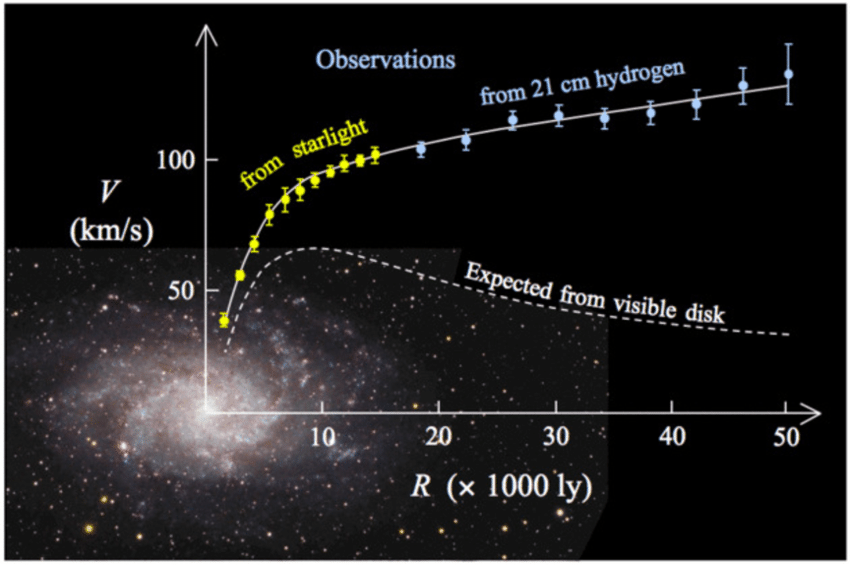
\includegraphics[width=0.75\textwidth]{figures/chapter_DM/M33-rotation-curve}
        \caption{
            Figure here shows the galactic rotational curve of M33, the expected rotational curve is shown in the dotted line. Experimental evidence observes behavior in the solid line.~\cite{M33}.
        }
        \label{fig:M33_figure}
    \end{center}
\end{figure}


\subsection{Gravitational Lensing}

    General relativity shows that massive objects would curve the space-time curvature around them. The details are capulated elegantly in the Einstein's Equation: 
%~\ref{eq:Einstein}: 

\begin{equation}
	R_{\mu \nu} - {1 \over 2}R \, g_{\mu \nu} + \Lambda g_{\mu \nu}= {8 \pi G \over c^4} T_{\mu \nu}, 
    \label{eq:Einstein}
\end{equation}

	In this equation, $R_{\mu \nu}$ is the Ricci curvature tensor, and R is the scalar curvature, together they form the Einstein tensor. $g_{\mu \nu}$ is the metric tensor, and $T_{\mu \nu}$ is the stress-energy tensor. This equation shows that the curvature of space-time is directly related to the mass and energy in that space. 	
	
	Consequentially, light rays that travel through the curved space-time around the massive object would therefore be bent. The effect mirrors that of angled lenses bending light rays due to a velocity difference of light rays across different media, and is called gravitational lensing. 

	There are different forms of lensing effect, roughly arranged by the strength of their effects. Strong lensing effect happens when bending of light result in either multiple images, a light ring or an arc, more typically observed around massive centers of galaxy clusters and galaxies; weak lensing usually involves statistical analysis of many objects over a large region; micro-lensing is detected when the effect only displays as an apparent change in the brightness of the source.

    Figure~\ref{fig:BulletCluster_figure} shows the bullet cluster collision of 1E 0657 -56. It is produced from the combination of gravitational lensing and x ray telescope imaging. The red part of the diagram denotes ordinary matter and the blue part reflects dark matter. In the cluster collision, ordinary matter bend light around them and became luminous from the collision, captured by x-ray imaging; the blue part shows a part of the clusters that did not interact and light up in the collision via gravitational lensing. This is a strong evidence for the existence of non-luminous matter in the clusters.

\begin{figure}[!htb]
    \begin{center}
        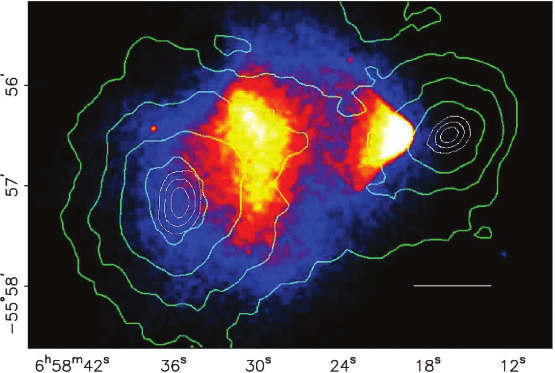
\includegraphics[width=0.75\textwidth]{figures/chapter_DM/BulletCluster}
        \caption{
			Bullet cluster (1E 0657-56) showing two colliding galaxy clusters, the part in red came from x-ray image by Chandra, highlighting normal matter distribution; the part in blue came from gravitational lensing. ~\cite{BulletCluster}.
        }
        \label{fig:BulletCluster_figure}
    \end{center}
\end{figure}


\subsection{Cosmic Microwave Background}

    In the beginning of the universe, ordinary matter and dark matter all exist in a hot plasma soup with frequent interaction between charged particles and photons through Thomson scattering. There comes a very important period in the universe called the recombination period, where the expansion of the universe has cool the plasma soup enough that charged particles began to form neutral atoms. Photons stopped scattering on the charged particles and went on unhindered. Due to red
shifting effect, they form a microwave background of the universe that can still be observed today. This is the Comic Microwave Background. 
This original background is nearly a black body and is therefore very uniform, but there exists small temperature variations. The variation can be decomposed into an angular power spectrum, as shown in Figure~\ref{fig:CMB_figure}

Due to the different interaction between dark matter and ordinary matter with photon and each other, simulation shows that different dark matter and ordinary matter make-up of the universe would result in different angular spectroscopy shape. 

Study from Planck on cosmic microwave background Figure~refgives a clear composition and percentage abundance of dark matter. Dark matter is not only an essential part of the universe, its composition is approximately 5 times as large as ordinary matter. Giving evidence that dark matter makes up the majority of the universe. 
%\figure planck 

\begin{figure}[!htb]
    \begin{center}
        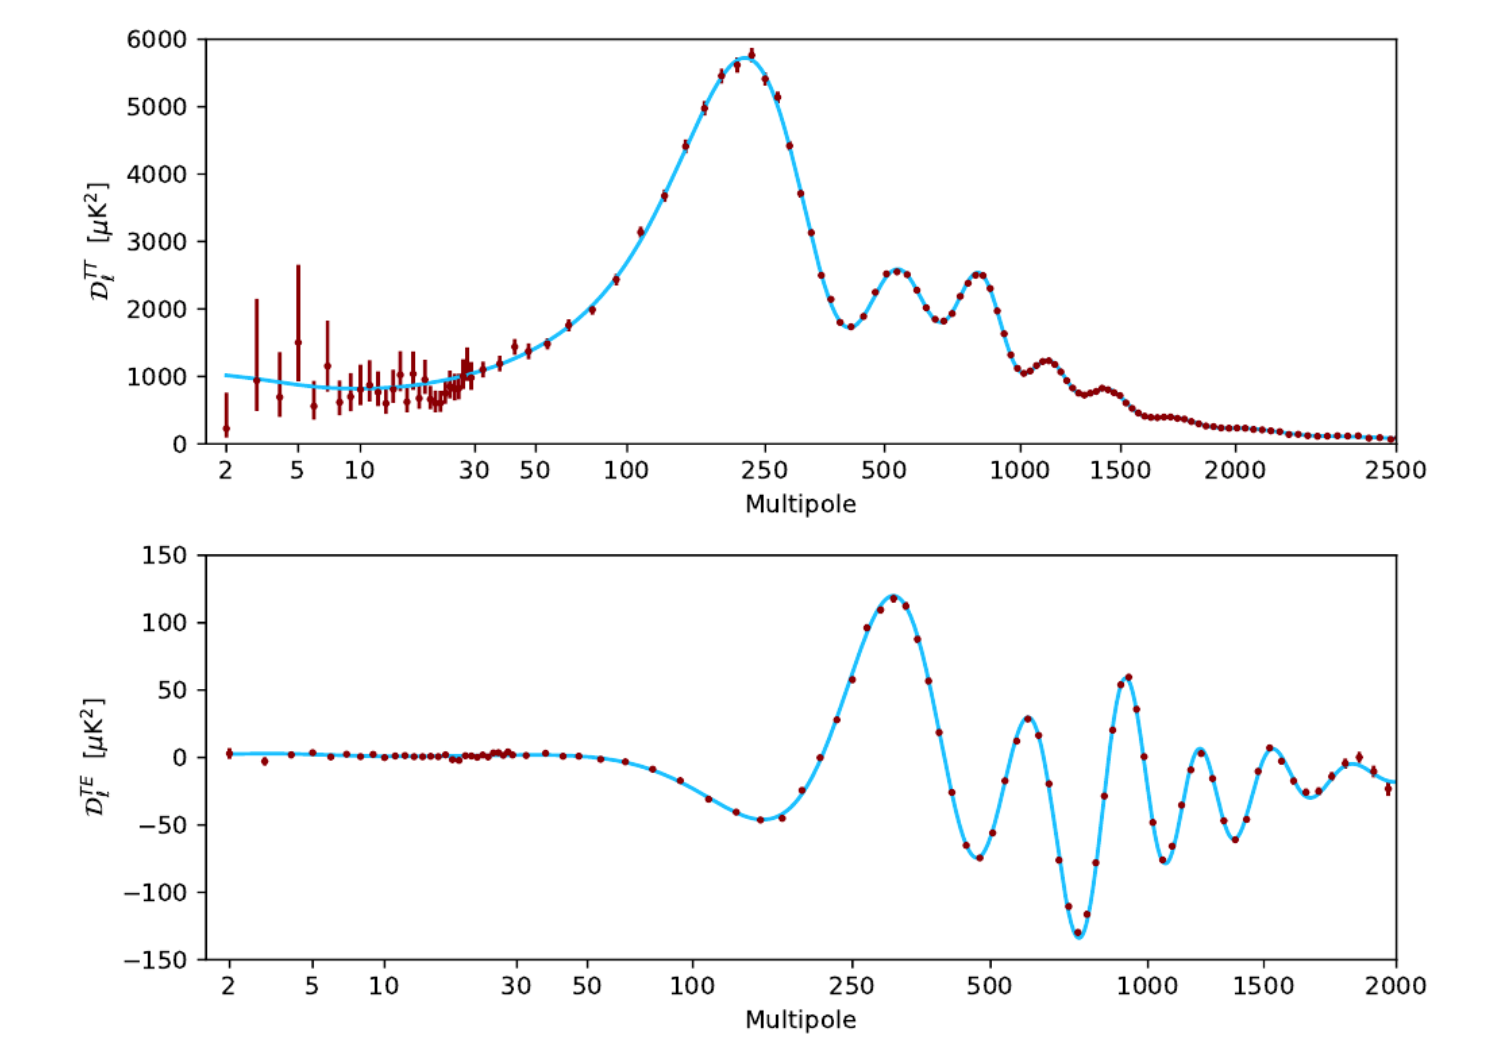
\includegraphics[width=0.75\textwidth]{figures/chapter_DM/CMB-angular-power-spectrum}
        \caption{
			The Cosmic Microwave Background power spectrum measured by Planck.~\cite{CMB}.
        }
        \label{fig:CMB_figure}
    \end{center}
\end{figure}


%\subsection{Large Scale Universe Structure}
%Gravity has a deterministic effect on how the universe is formed, and therefore affects the large scale structure of the universe. The existence of dark matter 
%https://www.forbes.com/sites/startswithabang/2020/10/02/ask-ethan-can-dark-matter-really-explain-the-universes-structure/?sh=5b37659b3b06


\section{Properties}
\label{section:properties}
While dark matter itself has never been directly observed, many studies in the cosmological, astrophysical and particle scale has constrained much of its properties. In this section and the remaining thesis, the following properties of dark matter will be assumed along with its justifications.

\subsection{Dark}

Dark matter got its name from its little to no interaction with light compared to ordinary matter in cosmological observation. Collision of the bullet cluster has also greatly constrained its interaction with itself.  
It is taken that it will not interact with collider detector and its interaction with ordinary matter would be rare in the energy scale of the LHC. 

\subsection{Long Life Time}

As dark matter is seen today in evidence across difference scales (see section ~\ref{section:evidence}). It is assumed to have a long life time since its creation in the early universe. Many theoretical model of dark matter require a $Z_{2}$ symmetry (such as the R parity of supersymmetry). This prevent dark matter particles from decaying into lighter Standard Model objects. In most experimental searches today, it is be treated as a single particle that does not decay further into other detectable SM particles. ~\cite{boveia2018dark}


\subsection{Interact Gravitationally}
Current evidence (see section ~\ref{section:evidence}) suggests that dark matter is massive (i.e. it interacts gravitationally). However, there is no consensus on the mass on the individual parts of dark matter. Current theoretical candidates of dark matter roughly be split into two camps: cold dark matter and hot dark matter. The former group believes that dark matter is made of object massive enough to be non-relativistic; the latter group hold the opposite view. 

\subsection{Cold}
In cosmology, hot/cold refers to the mass of an object. Only objects relatively low in mass would be affected relativistically. Different assumption of the relativistic mass of dark matter has great impact on the galaxy formations and its distribution. From most simulation results, dark matter is taken to be non-relativistic by most physicists and will be assumed for dark matter candidate searched for in the rest of the thesis. 

\subsection{Low Self-Interaction}
Dark matter is believe to have little to no self interaction, Mixed X-ray, optical and gravitational lensing study on the merging galacy cluster 1E-657-65 has restricted its self interaction limit to below $\sigma \over m < 1.25 cm^{2} g^{−1}$ (68\% confidence)~\cite{randall2008constraints}. 
 
%\subsection{Single Particle}
%While there are many composite dark matter models being proposed these days, dark matter is still taken to be a single kind in most effective model/simplified model building for experimental searches. 

\section{Candidates}
\label{section:candidates}

There exist a wide range of candidates for what dark matter could be. In here, a few possible particle candidate of dark matter are outlined here. 

\subsection{Sterile Neutrino}
Standard model does not predict that neutrino has a mass, however, that contradicting with experimental finding and is therefore a problem of the standard model. By replacing right-handed neutrinos in the standard model with gauge singlet fermions that has no interaction other than mixing with normal neutrinos, sterile neutrino is formed by theoretical models. Tuning parameters such its interaction rate with normal neutrino, mass and mixing angle, sterile neutrino can be a possible candidate for dark matter, as it can lead to a right
density of dark matter with stability consistent with the scale of the universe. ~\cite{dodelson1994sterile} They are searched for in radiator experiments such as the Daya Bay \cite{an2014search, wong2017search} and in scintillator experiments like DANSS. ~\cite{alekseev2018search}

% Mass and range  mass keV scale, currently sterile neutrino mass is unknown and therefore can be either hot or cold

%Daya Bay Collaboration, F. P. An et al., “Search for a Light Sterile Neutrino at Daya Bay,” Phys. Rev. Lett. 113 (2014) 141802, arXiv:1407.7259 [hep-ex].
%1310.8642
\subsection{Axion}
Another exisitng problem in the standard model is the strong CP problem. The strong CP problem points to the unnaturalness of CP symmetry observed in neutrons charge distribution measurement. This gives an exceptionally small value to the term that govern strong CP violation in the Standard Model, which is unnatural. The problem can be solved by introducing an additional axion particle and its associated fields to the standard model. ~\cite{peccei1977cp} With the proposition of such field, the CP violation term in strong interaction will be cancelled out naturally, thereby giving an explanation to the unnaturalness to the experimental value. 
The axion proposed is a dark matter candidate, as its calculated life time is much greater than the age of the universe and it shares many properties with the known profile of dark matter. Recent experimental finding from the XENON1T and shows anomalies that could be signs of axions. ~\cite{aprile2020excess}
%ADMX mass mu eV
%https://arxiv.org/pdf/2105.01406.pdf

%Xenon Collaboration, E. Aprile et al,. "Excess Electronic Recoil Events in XENON1T", Phys. Rev. D 102, 072004 (2020), arXiv: 2006.09721


% Non-particle candidates
%\subsection{Modified Newtonian Gravity}
%\subsection{MACHOs}

\subsection{Weakly Interacting Massive Particle (WIMP)}
A very attractive candidate for dark matter is called the weakly interacting massive particle(WIMP). It appears naturally with many Beyond-the-Standard-Model theories that aim to solve other physics problems, including theories of supersymmetry with R-parity and some extra dimensional theory. 
In the study of dark matter in cosmology, it is frequently assumed to be a thermal relic. Thermal relic dark matter is in thermal equilibrium with ordinary matter in the early universe. In thermal equilibrium with ordinary matter, it gets produced and annihilated at the same rate. There comes a point in the universe called freezing out, where the expansion of the universe cools the particle bath and produce temperature lower than possible to produce enough energy statistically for dark matter to
be produced given certain dark matter mass. Dark matter production from ordinary matter ceased. As the universe further expanse, it becomes more difficult for dark matter to find each other to be annihilated to form ordinary matter. Dark matter abundance is locked at this point and remained unchange until today. 
Using this model and the current measured abundance of dark matter in our current universe, the self annihilation cross section of dark matter is $ \langle \sigma \cdot v \rangle \simequal 3 \cdot 10^{26}cm^{3} s^{-1}$. This annihilation cross section scale matches many prediction made in supersymmetry theories. Many Beyond-the-Standard-Model theories, such as SUSY, the Universal Extra Dimension Model, and the little Higgs all predict a particle with known dark matter properties and self interaction rate of the same scale. This is known as the WIMP miracle. ~\cite{Dev_2014}

%\Figure WIMP miracle


\begin{figure}[!htb]
    \begin{center}
        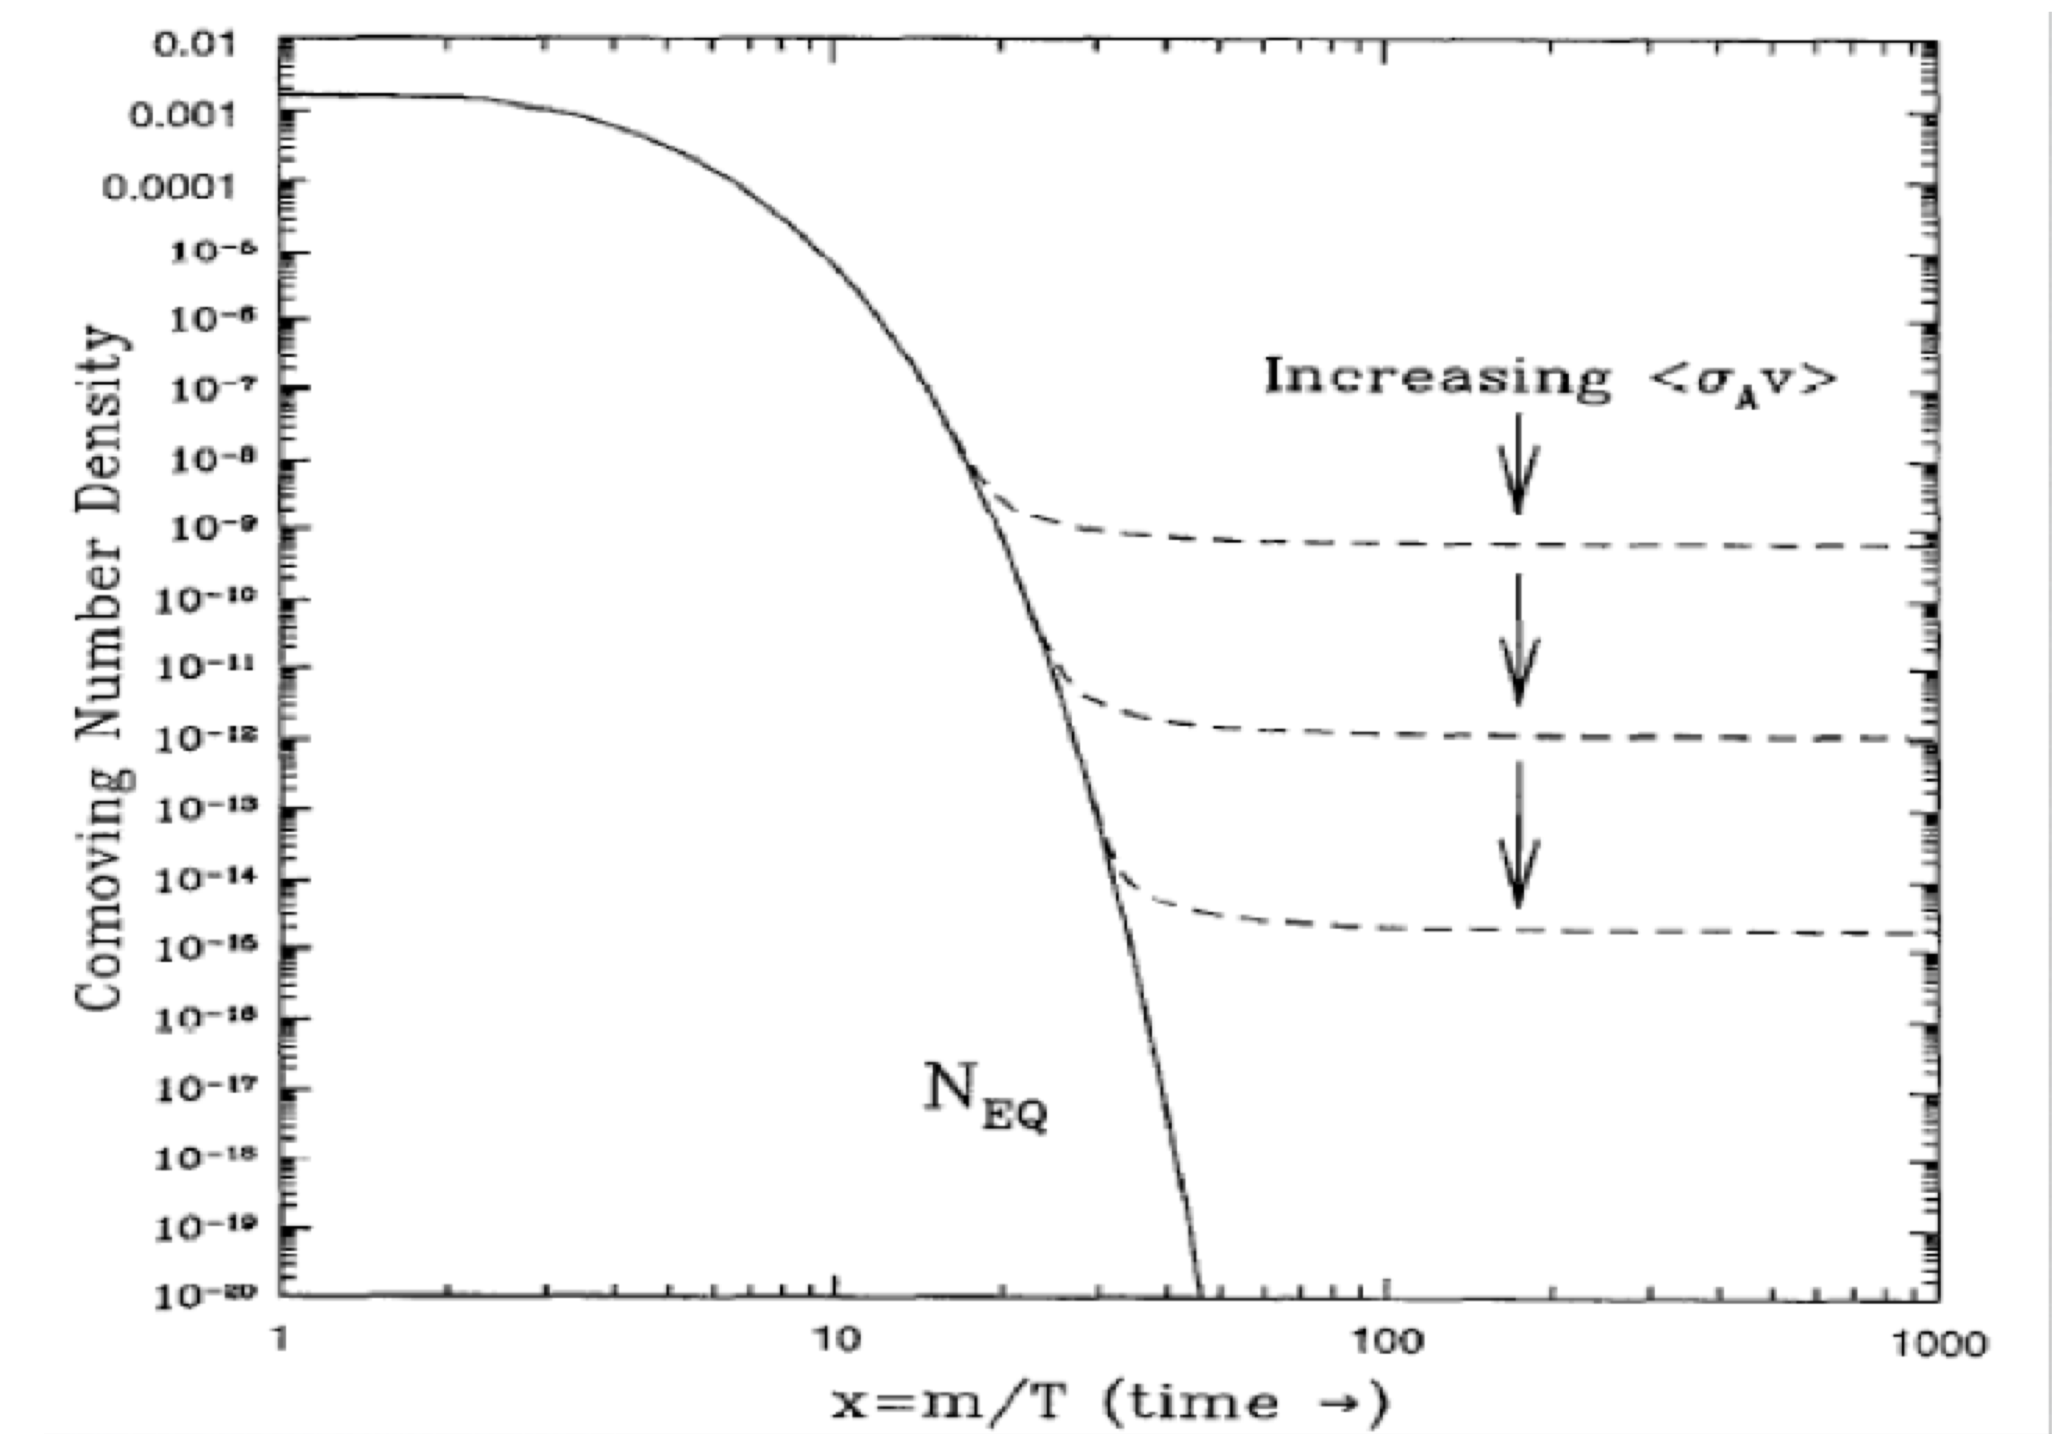
\includegraphics[width=0.75\textwidth]{figures/chapter_DM/WIMP}
        \caption{
		Solid line here shows the change in the densitiy of dark matter in an expanding unverse. In the early universe, the solid line is horizontal, indicating the time when dark matter production and annihilation is equal. The line gradually fall with increase of time when production rate began to decrease with the universe expansion. Later as the universe further expands, the annihilation stops as well and dark matter gets freezes out to different density level with different assumed self interaction annihilation rates.~\cite{WIMP}.
        }
        \label{fig:WIMP_figure}
    \end{center}
\end{figure}


 

%P.S. BHUPAL DEV, ANUPAM MAZUMDAR, & SALEH QUTUB, FRONT.IN PHYS. 2 (2014) 26
%https://indico.cern.ch/event/473000/contributions/1993414/attachments/1209863/1764345/tait-Aspen.pdf

%https://www.particlebites.com/?p=7004
%https://www.forbes.com/sites/startswithabang/2019/02/22/the-wimp-miracle-is-dead-as-dark-matter-experiments-come-up-empty-again/?sh=5ebc59f46dbc

\section{Experimental Search Overview}
\label{section:searches}

Traditionally the search for dark matter is split into different experimental categories sorted by the different detection methods from different dark matter/normal matter interactions. 

\begin{figure}[!htb]
    \begin{center}
        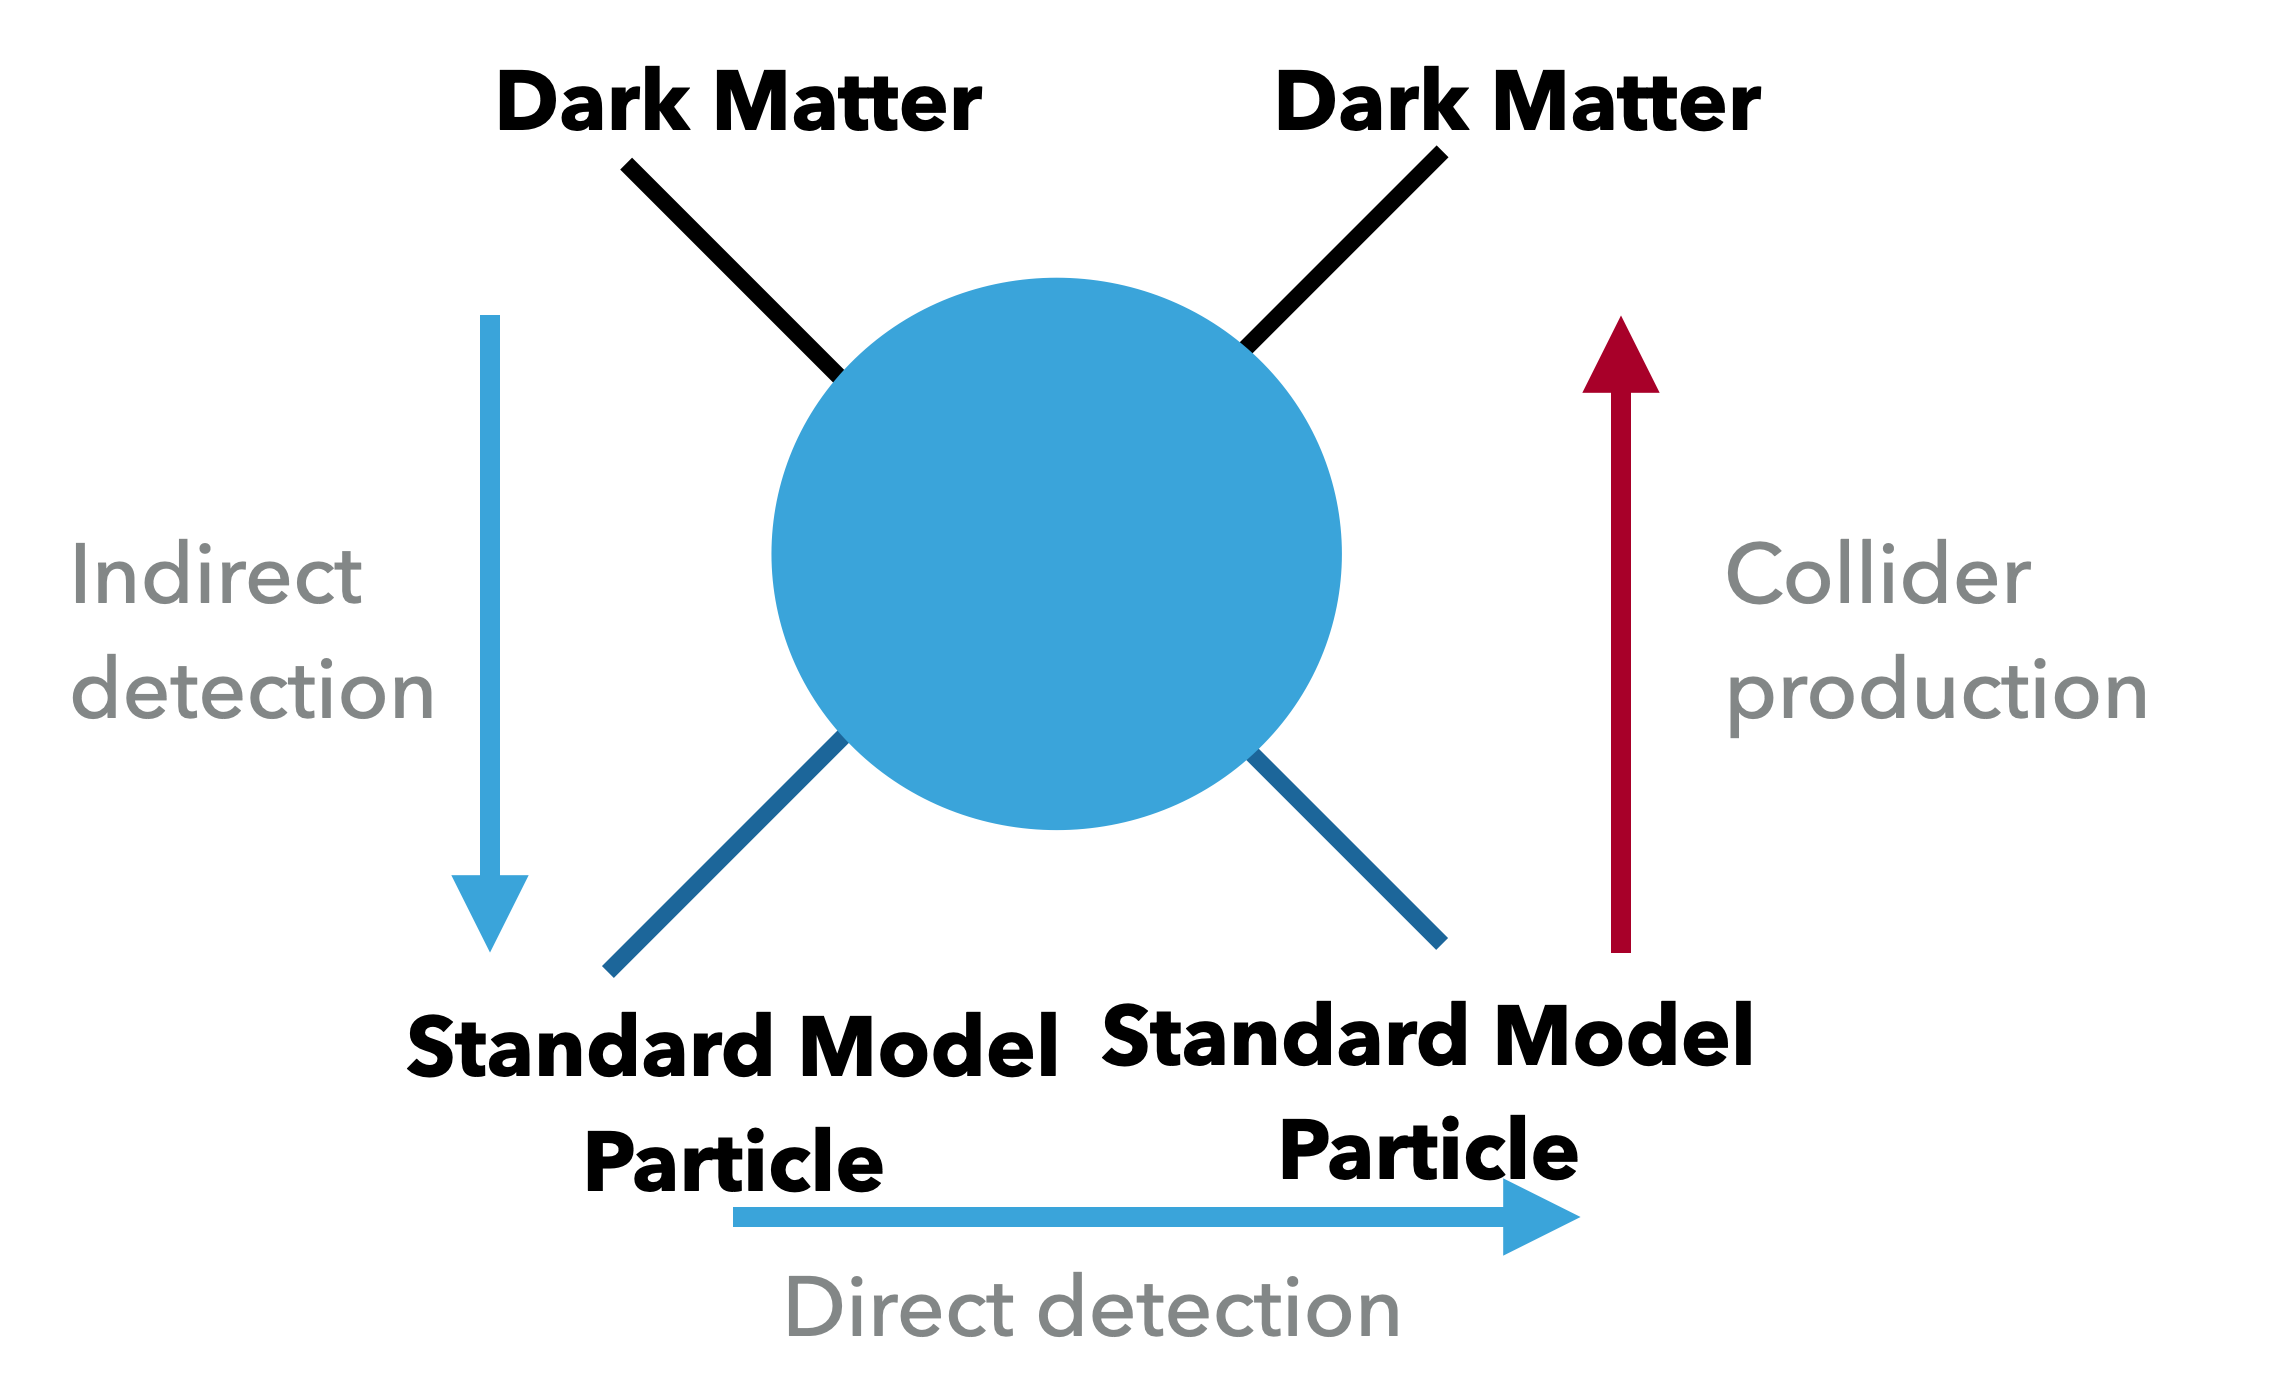
\includegraphics[width=0.75\textwidth]{figures/chapter_DM/Interaction}
        \caption{
			Schematic cartoon showing the different dark matter detection methods facilitated by different interactions thus signatures. 
        }
        \label{fig:interaction}
    \end{center}
\end{figure}

\subsection{Direct Detection}
Dark matter is believed to travel through the universe and passes through the eath. Assuming weak interaction between dark matter and Standard Model nucleons, dark matter can be detected directly with different target objects. 

\[ R \propto N \rho \chi \langle \sigma_{\chi } N \rangle \]

There are different experiments that uses different material and targets different dark matter masses.
Notable experiments include LZ ~\cite{mckinsey2016lz},   Xenon1T ~\cite{aprile2020excess}, SuperCDMS ~\cite{Agnese_2016}, CRESST ~\cite{Angloher_2014} and DAMA ~\cite{Bernabei_2008}. 

As more experiments has excluded much of the theory model phasespace, many of the experiments now faces the challenge of the neutrino floor in low mass dark matter search, which is where neutrino background began to dominate signal region. 



\subsection{Indirect Detection}
Indirect detection looks for annihilation Standard Model product of dark matter. It looks for interaction in places where matter is dense enough to interact, usually in center of galaxies and stars. Experiments include FermiLAT ~\cite{albert2017searching} and H.E.S.S. ~\cite{aharonian2006hess}


\subsection{Collider Production} 
    In the Large Hadron Collider, dark matter can be studied by being directly produced from Standard Model particles.

\section{Theoretical Models in LHC Searches}
\label{section:models}

While there exist a wide range of speculation on the identity of dark matter, the use of LHC as a dark matter searching tool constrains a unique set of dark matter candidate accessible phenomenologically. 
Focusing phenomenologically observable and interpretability for a wide range of theoretical models, different modeling approaches are used to develop benchmark models searching for dark matter in the LHC.
Sorting by an ascending degree of completeness, the literature will review different approaches and models of dark matter used in the LHC.


\begin{figure}[!htb]
    \begin{center}
        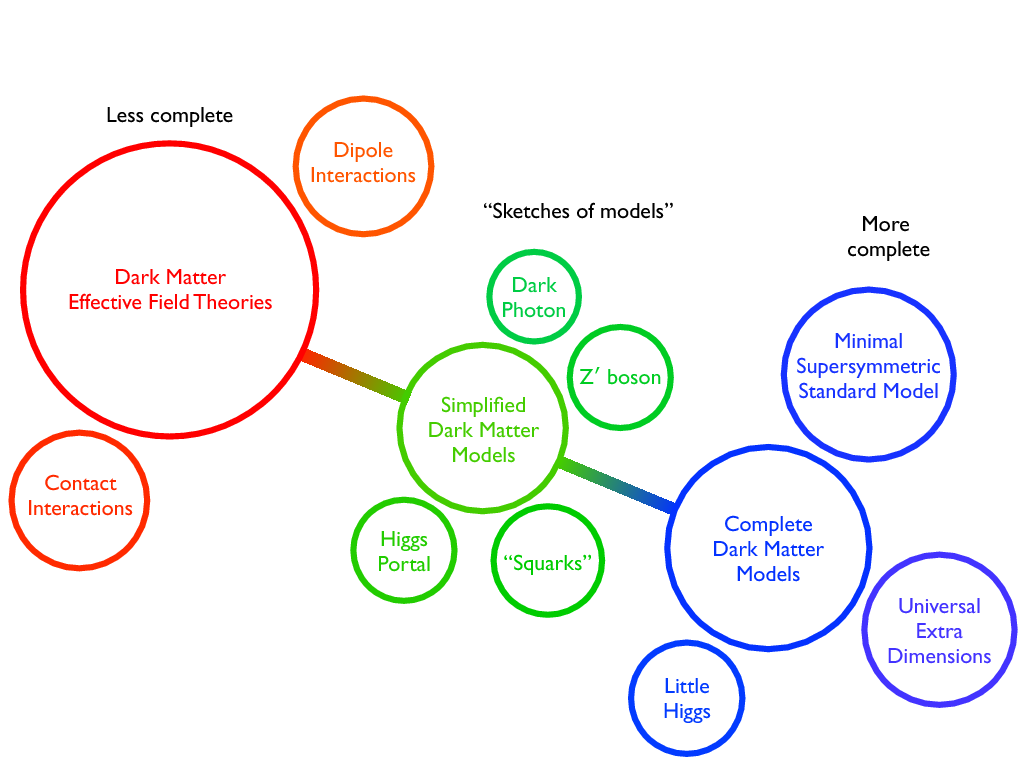
\includegraphics[width=0.75\textwidth]{figures/chapter_DM/Model}
        \caption{
			Colored Scheme showing dark matter modeling approach from more simplistic (left) to more complete models (right).  ~\cite{Abdallah:2024101}.
        }
        \label{fig:Model_figure}
    \end{center}
\end{figure}



\subsection{Simple Portal Models}
The simplest kind of models are simple extensions to the standard model. In these models, dark matter is mediated either through the Higgs or the Z Boson. As the Z portal models are constrained by LEP and DD experiments, dark matter that are mediated through a heavier version of Z boson ( the Z') and additional scalar is also searched for. 

\subsection{Effective Field Theory}
The effective field theory approach condenses a wide range of complete models to simplified versions by focusing on what is experimentally accessible. High mass mediator particles in complete theories as a contact operator. High energy correction and details are integrated out for "effectiveness". All kinematically accessible observables are described by a Lorentz structure and a rate parameter. 
This approach allow for the easily measured experiment values and a framework for a wide range of complete models to be probe with few experimental model search. However, the model has a singularity and is not valid for when the interaction momentum transfer is close to that of the mediator mass. In the LHC, a truncation method is used to bound the events simulated Monte Carlo events below this limit ~\cite{Busoni_2014}.

\subsection{Simplified Model}
The problem in effective field theory can be resolved with the simplified Model appraoch. The contact interaction in EFT is turned into mediator particle s-channel/t-channel exchanges in simplified model. With the price of an increased number of parameters, simplified models can provide the full mechanics of a particle interaction and usually come with more details. 
Simplified models of dark matter in the LHC do not break the global and gauge symmetries of Standard Model, the Lagrangian terms are Lorentz invariant and predicts at least a dark matter candidate that fullfills the properties described in the previous section. 
Some simplified dark matter model used in the LHC include the Two-Higgs Doublet Model (2HDM), where Higgs or a non-standard model exotic Higgs could serve as a mediator to dark matter; other examples include dark photon or a kinetically mixed Z' dark matter model. 
Other than these, simplified model in supersymmetry such as the Phenomenological Minimal Supersymmetric Standard Model (pMSSM) which reduces the over 100 parameters of complete model of Minimal Supersymmetric Standard Model to 19 parameters, predicts candidate dark matter like particles, predicts neutralino as a natural dark matter candidate. 
In addition, other gauge or gravity mediated SUSY theory predicts gravitino as a dark matter candidate. 
% pMSSM Assumes no sources of CP violation Beyond-the-Standard-Model and no flavor-changing neutral currents, and retains uni- versal couplings and masses for first- and second-generation superpartners. %CatDog Antonio DM summary paper.  

\subsection{Less-simplified models}
The LHC dark matter working group is moving towards less simple models with more phenomenological details.
%\subsection{Long-Lived Particle Models}

A detailed list of models used by the LHC by both the CMS and ATLAS can be found in this reference ~\cite{Abercrombie_2020}.

\section{Experimental Signature in the LHC}
\label{section:signatures}

\subsection{Mono-X signature}
    This describes the type of dark matter search where an invisible dark matter is produced directly in the LHC and is "observed" in the detector as missing transverse momentum.
    Dark matter is known to interact only very weakly with normal matter, and thus is assumed to not leave a trace in the LHC detector. When events are produced through proton-proton collision along the z-axis in the LHC, the momentum of all objects along the transverse plane to the z-axis is always zero. Therefore, when an event has missing transverse momentum recoiling against another visible object, the signature would possibly be dark matter.
This class of analysis is named by the standard model object that dark matter recoil against. Mono-jet, mono-Higgs, mono-Z are a few analyses done this way. 

\subsection{Di-object Signature}
    Dark matter can also be searched for without the production of the dark matter particle. The simplified models that predicts dark matter in the mono-X analyses predicts effective mediator particle between standard model particle with dark matter. These effective mediator particles can be directly searched for through via decay back into standard model object. As the process is distinct from any known Standard Model particle processes, an excess of events Beyond-the-Standard-Model prediction for
    such a mediator process could be evidence for dark matter in the LHC. 
These di-object search include dijet, dilepton, diphoton searches. 
In recent years, new techniques such as the trigger-level-analysis and channels that has an additional initial state radiation objects are being pioneered. These result in a search phasespace much greater than the traditional program and greatly extended the of the richness of the LHC serach program.

\subsection{Supersymmetric Signature}	

\subsection{Long-Lived Particle Signature}

